\documentclass[a4paper,12pt]{article}
\usepackage[utf8]{inputenc}
\usepackage[cm,empty]{fullpage}
\usepackage[T2A]{fontenc}
\usepackage[english, russian]{babel}
\usepackage{amssymb,amsmath,amsxtra,amsthm}
\usepackage{proof}
\usepackage[pdftex]{graphicx}
\usepackage{wrapfig}

\usepackage[dvipsnames]{xcolor}

\usepackage[left=2cm,right=2cm,
    top=1cm,bottom=1cm,bindingoffset=0cm]{geometry}

\renewcommand{\leq}{\leqslant}
\renewcommand{\geq}{\geqslant}


\newcommand{\iiff}{\Longleftrightarrow}
\renewcommand{\iff}{\Leftrightarrow}
\newcommand{\nothing}{\varnothing}

\newtheorem*{rem}{Замечание}

\newcommand{\NN}{\mathbb{N}}
\newcommand{\ZZ}{\mathbb{Z}}
\newcommand{\Q}{\mathbb{Q}}
\newcommand{\A}{\mathbb{A}}
\newcommand{\R}{\mathbb{R}}
\renewcommand{\C}{\mathbb{C}}

\renewcommand{\phi}{\varphi}
\newcommand{\eps}{\varepsilon}

\newcounter{z}


\newcommand{\z}{\refstepcounter{z}\vskip 20pt\noindent
\fbox{\textbf{\arabic{z}}} }

\newcommand{\zs}{\refstepcounter{z}\vskip 20pt\noindent
\fbox{\textbf{\arabic{z}$^{^\circ}$}} }



\renewcommand{\date}{{\bf 9 декабря 2020}} %Дата занятия

\newcommand{\dif}
{
------------------------------------------------------------------------------------------------------------------------------------------------------
}

\newcommand{\HSEhat}{
\vspace*{-0pt}
\noindent
\setcounter{z}{0}
\vspace*{-10pt}
\begin{wrapfigure}[2]{l}{5pt}
\vspace*{-25pt}
\hspace*{-20pt}

\includegraphics[scale=0.18]{img/HSE_LOGO.png}
\end{wrapfigure}
\vspace{-20pt}


{\bf \phantom{\date}  \large \hfill Дискретная математика: \hfill \normalsize \date}

\vspace{5 pt}
{\bf \large \hfill  ориентированные графы и алгоритмы на графах.\hfill }



\vspace*{10pt}
\setcounter{z}{0}

}

\begin{document}

\HSEhat


\setcounter{z}{5}

\zs Рассмотрим алфавит, состоящий только из двух букв $a$ и $b$. Все возможные слова, которые можно получить в этом алфавите, назовем языком.\\
Докажите, что в этом языке есть слово, в котором любая двухбуквенная комбинация ($aa$, $ab$, $ba$, $bb$) встречается ровно один раз.\\

\begin{proof}
Составим граф $G$, вершинами которого будут все слова длины $2$. Соединим ориентированным ребром два слова $w_1$ и $w_2$, если последняя буква $w_1$ совпадает с первой буквой $w_2$ (например, в нашем графе будет ребро $(ab,ba)$, т.е. $ab \to ba$). Граф можно увидеть на левом рисунке.

\begin{center}
    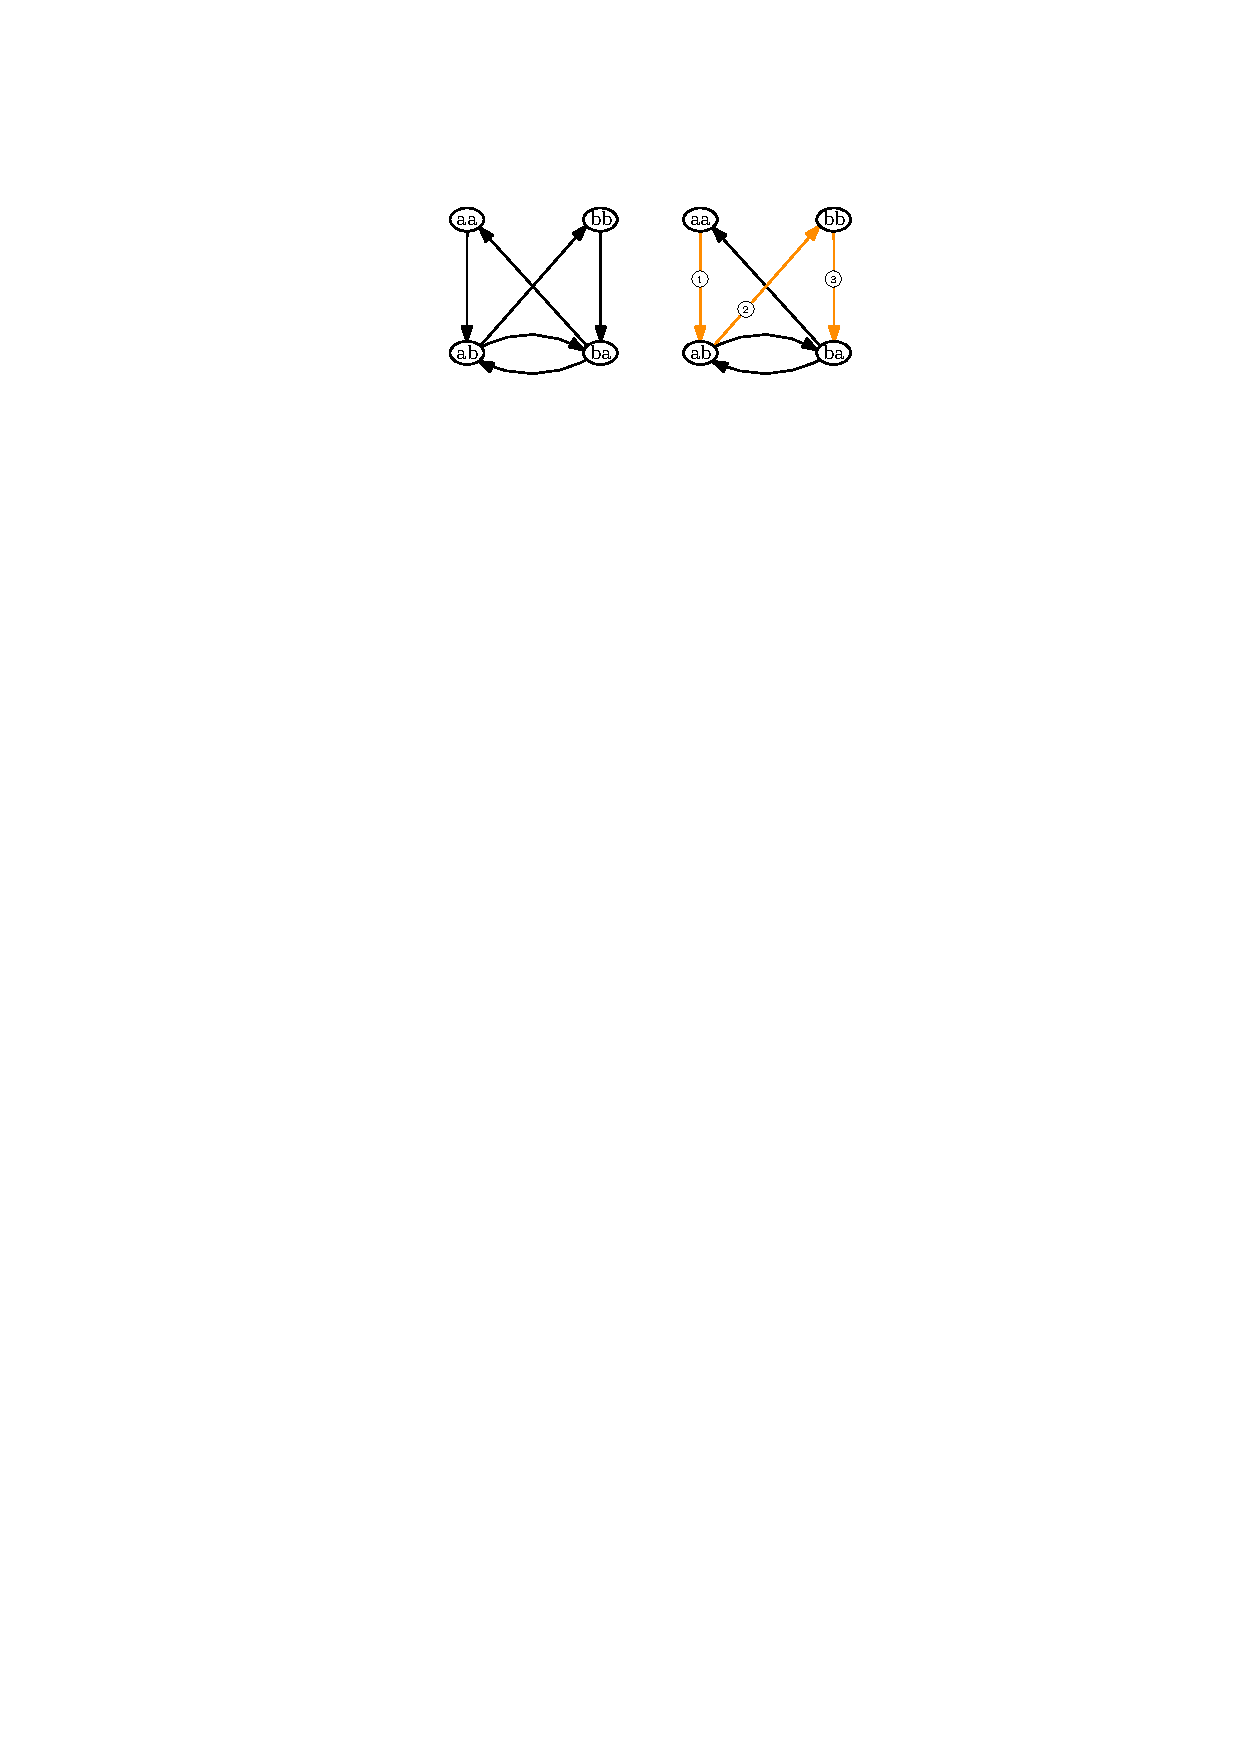
\includegraphics[width=0.8\textwidth]{img/digraphHW6.pdf}
  \end{center}

Если слова соединены ребром, то их можно написать подряд с пересечением последней и первой буквы ($\textcolor{Maroon}{a}\textcolor{ForestGreen}{b} \to \textcolor{ForestGreen}{b}\textcolor{RoyalBlue}{a}$ дает слово $\textcolor{Maroon}{a}\textcolor{ForestGreen}{b}\textcolor{RoyalBlue}{a}$). Таким образом, путь образует слово, в котором поочередно идут двухбуквенные комбинации, соответствующие вершинам  этого пути ($ab,ba,ab,bb$ дает слово $ababb$).

Тогда слову, в котором любая двухбуквенная комбинация встречается ровно один раз, соответствует путь, проходящий по всем вершинам ровно один раз. 

Таким является, например, $aa,ab,bb,ba$. Он дает слово $aabba$, в котором действительно любая двухбуквенная комбинация встречается ровно один раз.

Ответ: $\mathbf{aabba}.$

\end{proof}

\end{document}